\documentclass[a4paper,12pt]{article}
\usepackage[utf8]{inputenc}
\usepackage{geometry}
\usepackage{graphicx}   % images
\usepackage{fancyhdr}   % headers/footers
\usepackage{tcolorbox}
\usepackage{listings}
\usepackage{xcolor}
\geometry{margin=1in}

% ---------- Header ----------
\setlength{\headheight}{36pt}
\setlength{\headsep}{18pt}
\renewcommand{\headrulewidth}{0.4pt}
\fancyhf{}
\fancyhead[L]{
\includegraphics[width=0.13\textwidth, keepaspectratio]{Figures/UM6Plogo.png}}
\fancyhead[R]{
\includegraphics[width=0.13\textwidth, keepaspectratio]{Figures/CC.jpg}}
\fancyfoot[L]{Data Management Lab}
\fancyfoot[R]{Prof.\ Karima Echihabi}
\fancyfoot[C]{Page \thepage}

% ---------- Deliverable Template ----------
\begin{document}
\thispagestyle{empty}
\begin{center}
  
\includegraphics[width=0.25\textwidth]{Figures/UM6Plogo.png}\hfill
  
\includegraphics[width=0.25\textwidth]{Figures/CC.jpg}
  \vspace{1.2cm}

  {\LARGE \textbf{Deliverable \#: \\[0.5cm] Moroccan National Health Services (e.g.: Conceptual Design ....)}}\\[0.6cm]
  {\large \textbf{Data Management Course}}\\[0.2cm]
  {\large UM6P College of Computing}\\[0.8cm]

  {\normalsize \textbf{Professor:} Karima Echihabi \quad 
   \textbf{Program:} Computer Engineering}\\[0.1cm]
  {\normalsize \textbf{Session:} Fall 2025}\\[1cm]

  \rule{0.9\textwidth}{0.5pt}\\[0.5cm]
  {\large \textbf{Team Information}} \\[0.3cm]
  \begin{tabular}{|l|l|}
    \hline
    \textbf{Team Name} & Index Five \\ \hline
    \textbf{Member 1}  & Zakarya Aze-Dine  \\ \hline
    \textbf{Member 2}  & Adam Ajerouassi   \\ \hline
    \textbf{Member 3}  & Youssef Benhammouda   \\ \hline
    \textbf{Member 4}  & Adam Biar   \\ \hline
    \textbf{Member 5}  & Yahia Belefquih   \\ \hline


    \textbf{Repository Link} & \texttt{https://github.com/Youssefbenhammouda/DBMS-IndexFive} \\ \hline
  \end{tabular}
  \rule{0.9\textwidth}{0.5pt}\\
\end{center}
\clearpage
\pagestyle{fancy}

% ---------- Sections for Students ----------
\section{Introduction}
The Moroccan National Health Services (MNHS) requires a comprehensive database to manage patient care, staff operations, hospitals, appointments, prescriptions, medications, insurance, billing, and emergencies. This deliverable provides the Entity–Relationship (ER) model for the MNHS system. It captures the main entities, their attributes, and relationships to support both operational queries (e.g., patient admission, prescription tracking) and future analytics (e.g., staff workload, medication demand). The ERD ensures data consistency, supports scalability, and aligns with healthcare management requirements in Morocco.
\section{Requirements}
This deliverable covers:
\begin{itemize}
    \item Patient management (personal info, insurance, address, phone, history).
    \item Staff management (practitioners, caregiving staff, technical staff, certifications).
    \item Hospital and department management (region, city, wards, specialties).
    \item Appointment scheduling (patient, staff, department, time, reason).
    \item Prescription handling (doctor, dosage, duration, medication).
    \item Medication inventory (pharmacy stock, suppliers, prices, restock dates).
    \item Insurance and billing management.
    \item Emergency cases and triage management.
    \item Linking hospitals, departments, and services under MNHS.
\end{itemize}



\section{Methodology}
Below we explain each entity and its relationships, with cardinalities. 
In our notation: 
\begin{itemize}
    \item \textbf{Bold line} = $(1 \dots N)$ 
    \item Normal line = $(0 \dots N)$
    \item \textbf{Bold Arrow} = $(1)$ 
    \item Normal Arrow = $(0,1)$
\end{itemize}

\subsection*{Patient}
Attributes: \texttt{internal\_id}, \texttt{full\_name}, \texttt{CIN}, \texttt{sex}, \texttt{birth\_date}, \texttt{blood\_grp}.  
\begin{itemize}
    \item Aggregation: grouped with \texttt{Location} (province, city, street, postal code) and \texttt{Phone}.  
    A patient may have $0\dots N$ locations and each one of them has one phone.
    \item Relation with \texttt{Insurance}: a patient can have $1\dots N$ insurances.
    \item Relation with \texttt{Emergency}: a patient can be admitted in $0\dots N$ emergencies.
    \item Relation with \texttt{Appointment}: a patient can have $0\dots N$ appointments, each appointment must involve exactly $1$ patient.
    \item Relation with \texttt{Prescription}: a patient can have $0\dots N$ prescriptions.
\end{itemize}

\subsection*{Insurance}
Attributes: \texttt{insur\_id}, \texttt{coverage\_type}.  
\begin{itemize}
    \item Each insurance must be linked to $0\dots N$ patient.
    \item An insurance can have $0\dots N$ bills.
\end{itemize}

\subsection*{Bill}
Attributes: \texttt{bill\_id}, \texttt{generation\_time}.  
\begin{itemize}
    \item A bill can be attached to exactly $1$ insurance. 
\end{itemize}

\subsection*{Appointment}
Attributes: \texttt{app\_id}, \texttt{date}, \texttt{time}, \texttt{status}, \texttt{reason}.  
\begin{itemize}
    \item Each appointment must be linked to exactly $1$ patient.
    \item Each appointment must be linked to exactly $1$ staff.
    \item Each appointment must be linked to exactly $1$ department.
    \item Patients, staff, and departments may have $0\dots N$ appointments.
\end{itemize}

\subsection*{Staff (Hierarchy)}
Attributes: \texttt{staff\_id}.  
Specializations (hierarchy):
\begin{itemize}
    \item \texttt{Practitioners}: license number, specialty.
    \item \texttt{Caregiving staff}: ward, grade.
    \item \texttt{Technical staff}: modality/equipment.
\end{itemize}

Relations:
\begin{itemize}
    \item \texttt{work\_in}: each staff must belong to exactly $0\dots N$ department. A department may have $0\dots N$ staff.
    \item \texttt{Handles}: staff can handle $0\dots N$ emergencies. An emergency can be handled by $0\dots N$ staff.
    \item \texttt{has\_cert}: staff can have $0\dots N$ certifications. Each certification must belong to $0$ or $1$ staff.
    \item \texttt{Appointment}: each appointment must be linked to exactly $1$ staff.
    \item \texttt{Prescription}: each prescription must be issued by $0\dots N$ staff.
\end{itemize}

\subsection*{Department}
Attributes: \texttt{dept\_id}, \texttt{name}.  
\begin{itemize}
    \item Each department must belong to exactly $1$ hospital. A hospital can have $0\dots N$ departments.
    \item Staff and appointments are linked to departments as described above.
\end{itemize}

\subsection*{Hospital}
Attributes: \texttt{hos\_id}, \texttt{name}, \texttt{city}, \texttt{region}.  
\begin{itemize}
    \item Each hospital must have $1\dots N$ pharmacy inventory.
    \item A hospital may have $0\dots N$ departments.
\end{itemize}

\subsection*{Pharmacy Inventory}
Attributes: \texttt{phar\_id}.  
\begin{itemize}
    \item Relation with \texttt{Medication}: an inventory can contain $0\dots N$ medications.  
    Relationship attributes: quantity, unit price, reorder level, last restock timestamp.
\end{itemize}

\subsection*{Medication}
Attributes: \texttt{drug\_id}, \texttt{name}, \texttt{strength}, \texttt{form}, \texttt{active\_ingredient}, \texttt{manufacturer}, \texttt{therapeutic\_class}.  
\begin{itemize}
    \item May be contained in $0\dots N$ inventories.
    \item Must be included in $0\dots N$ prescriptions.  
    Relationship attributes: dosage, duration.
\end{itemize}

\subsection*{Prescription}
Attributes: \texttt{prescrip\_id}, \texttt{date}.  
\begin{itemize}
    \item Must be linked to $0\dots N$ patient.
    \item Must be linked to exactly $0\dots N$ staff.
    \item Must include $0\dots N$ medications.
\end{itemize}

\subsection*{Emergency}
Attributes: \texttt{emerg\_id}, \texttt{triage\_id}, \texttt{admission\_timestamp}, \texttt{outcome}.  
\begin{itemize}
    \item Must involve by $0\dots N$ patient.
    \item Can be handled by $0\dots N$ staff.
\end{itemize}

\subsection*{Certifications}
Attributes: \texttt{cert\_id}.
\begin{itemize}
    \item Each certification must belong to exactly $0$ or $1$ staff.
\end{itemize}
\section{Implementation \& Results}
\begin{figure}[htbp]
    \makebox[\textwidth][c]{%
        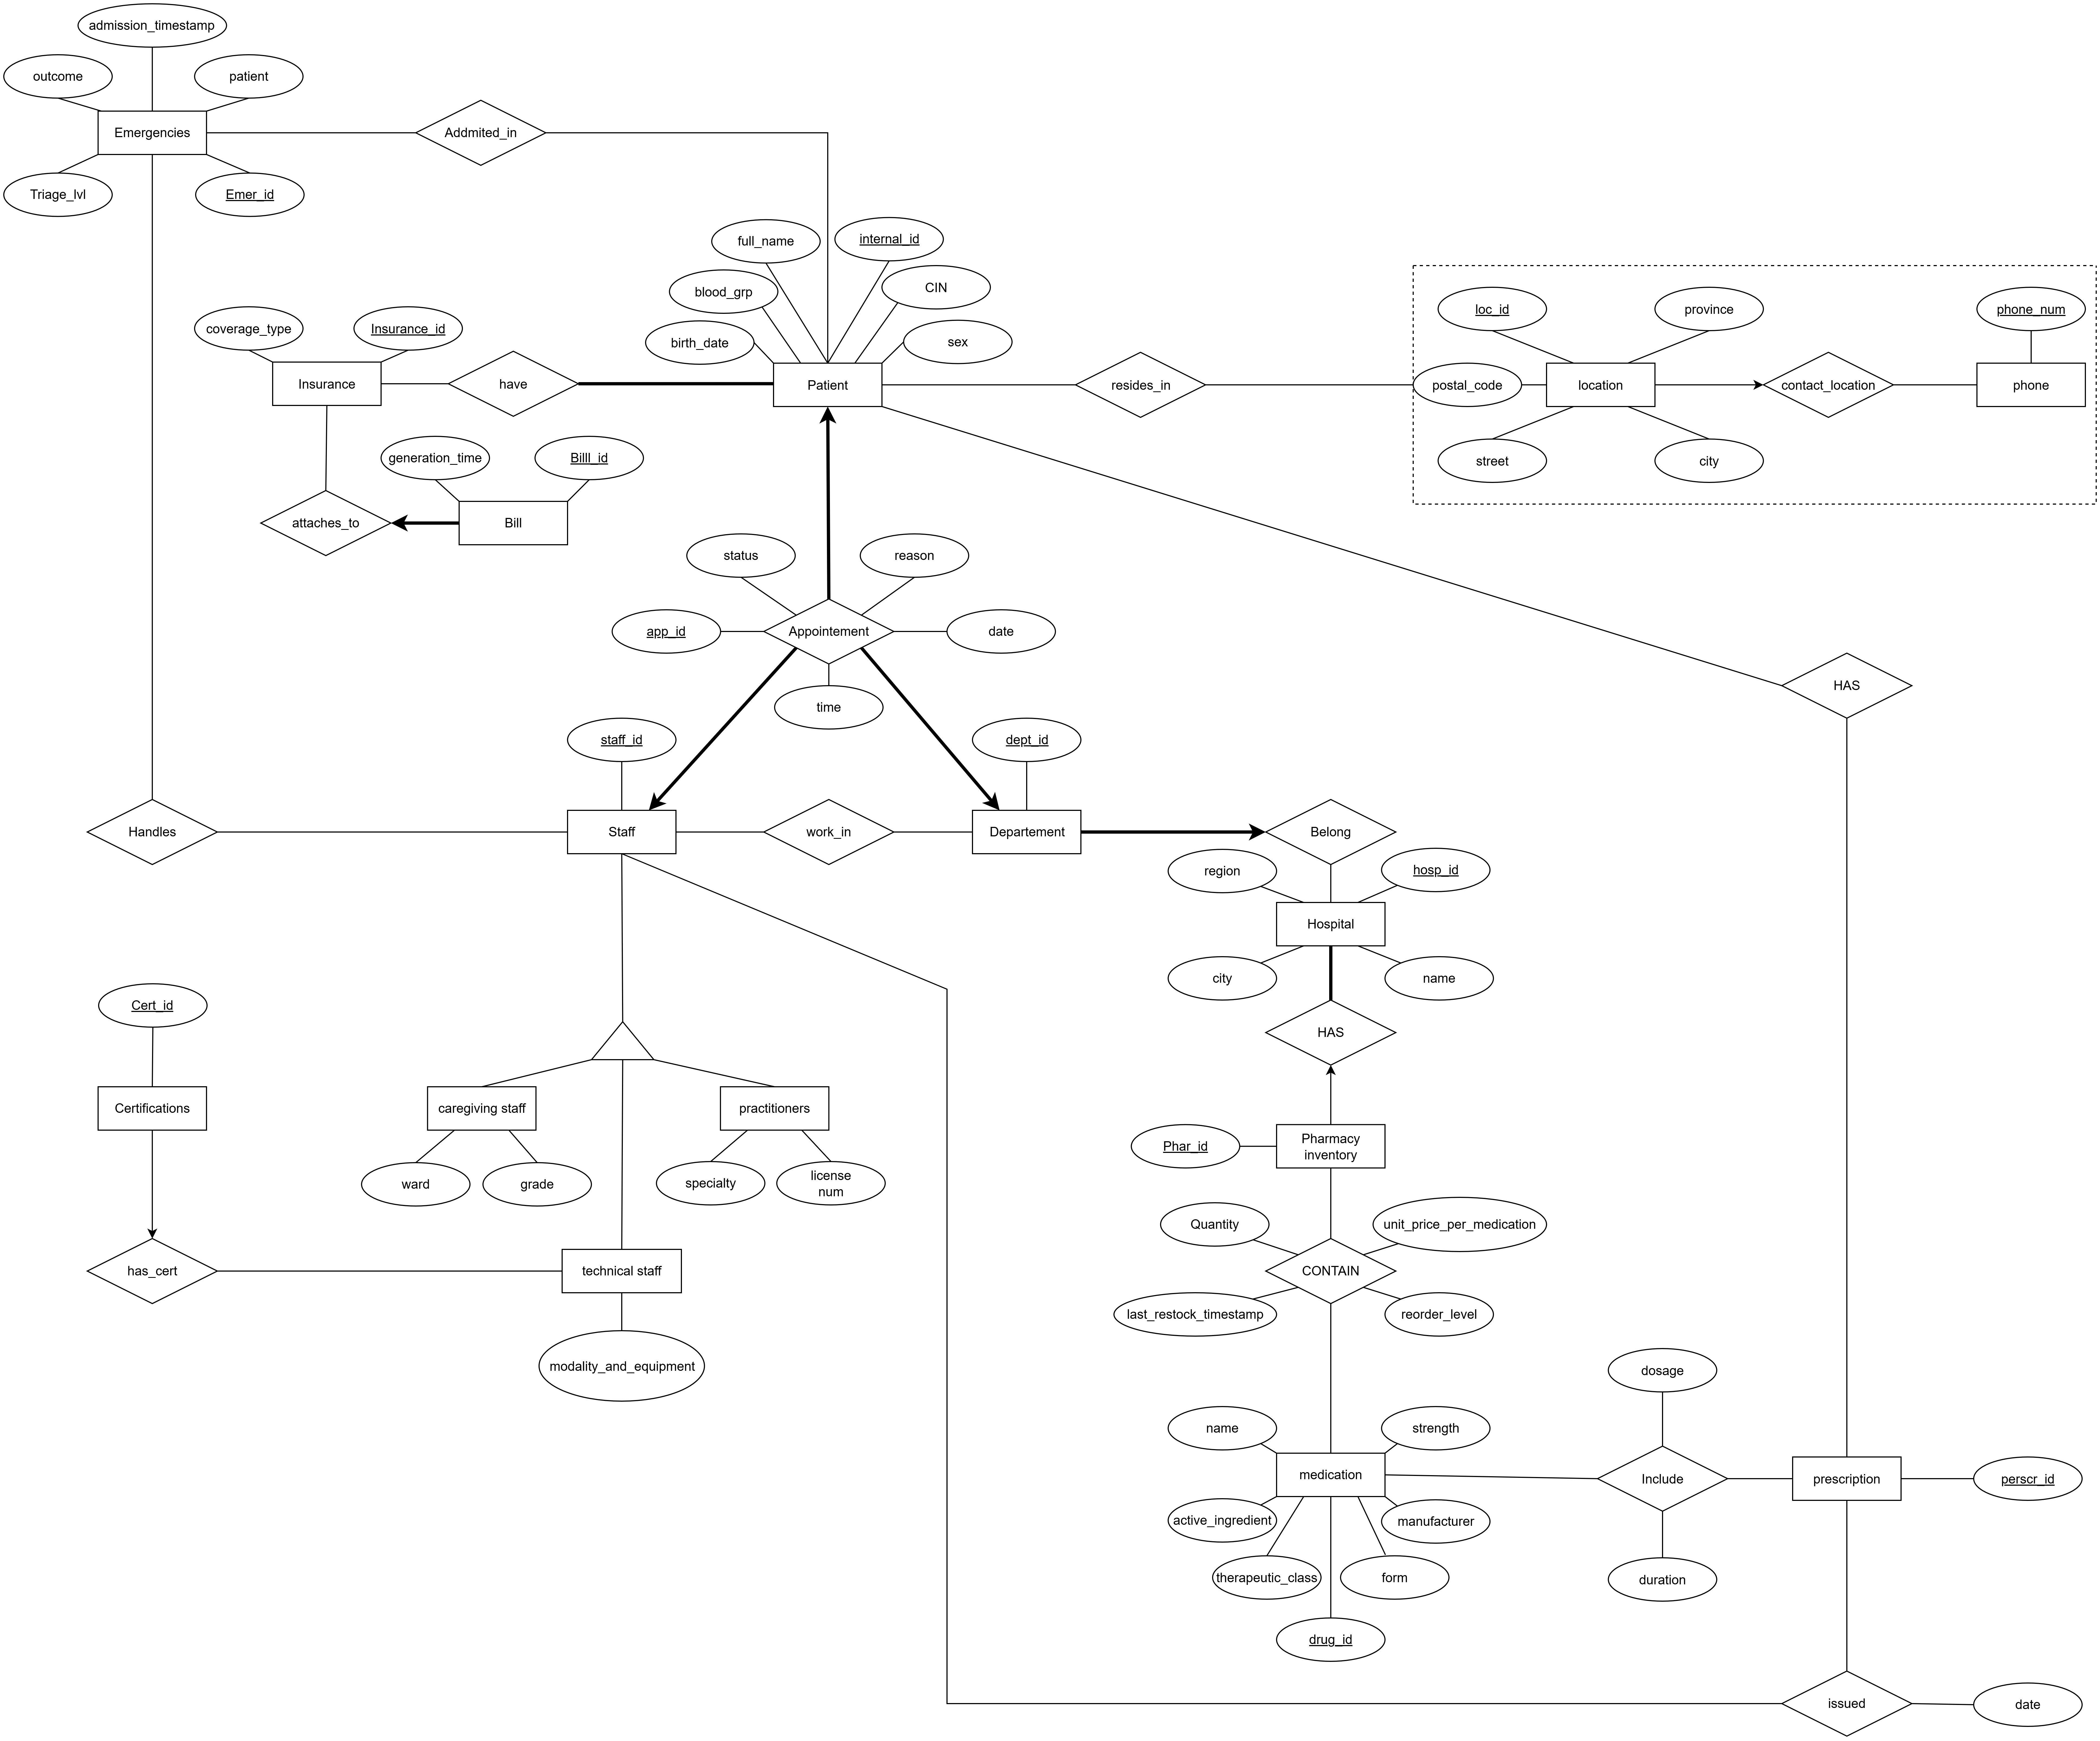
\includegraphics[width=1.15\textwidth]{figures/ERD.png}}
    \caption{ER Diagram}
    \label{fig:ERD}
\end{figure}

\newpage


\section{Discussion}
\textbf{Challenges faced}:
The challenges we encountered are:
Modeling the precription system .Since each prescription
can include multiple medications and each medication needs its own dosage and duration details.
To solve that,we had to create a specific relationship structure to capture this complexity.
The emergency section also posed questions:should we require staff assignment for every emergency,or allow for cases where this Information
might be missing ?

\textbf{Observations}:
During the designing process, it became evident that the nature of relationships within the healthcare domain was by nature complex, particularly many-to-many relationships between entities like patients and staff with multiple appointments, and prescriptions and associated multiple medications. We added time with various components—appointment time, duration of the prescription, and timestamps for emergencies—as notable components needing accurate modeling to support report accuracy and operations. Further, we needed to interweave varying staff roles into one structure (practitioner, caregiver, technical staff), indicating the need for a design that was both flexible and exact for all entities. Through our process, we observed and confirmed clinical databases must balance detailed transactional tracking with the need to facilitate a high-level analytic questioning.

\textbf{lessons learned}:
Through this project,we recognized that database design strikes the right balance between theoretical perfection and real-world uusability.
By defining ralationship constraints(e.g.specifying that each staff member belongs to one department while a department can contain many staff ).
Most significantly,we understood the importance of designing database not only for present operational needs but also for future scalability by supporting analytics and expansion.

\section{Conclusion}
This deliverable presents a complete conceptual design for the MNHS database system by creating an Entity-Relationship(ER) diagram between all the healthcare entities with their attributes and their realationships.
The design follows the project requirements while establishing a scalable foundation for both operational efficiency and future analytical needs


\end{document}
